\scanpage{42}
\figure{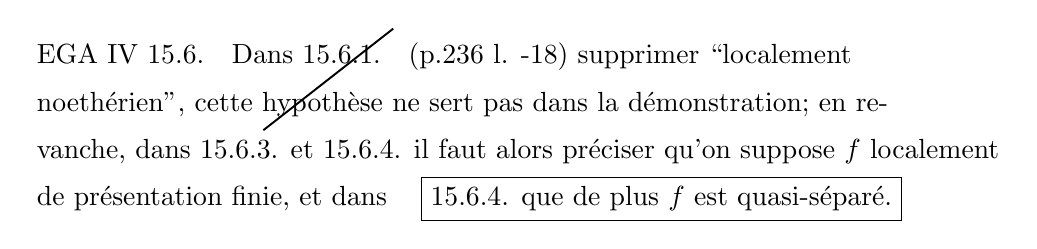
\begin{tikzpicture}[x=1cm,y=1cm]
\node[anchor=west] at (0,0) {EGA IV 15.6.\quad Dans 15.6.1.\quad (p.236 l. -18) supprimer ``localement};
\node[anchor=west] at (0,-.6) {noethérien'', cette hypothèse ne sert pas dans la démonstration; en re-};
\node[anchor=west] at (0,-1.2) {vanche, dans 15.6.3. \inserted{et 15.6.4.} il faut alors préciser qu'on suppose $f$ localement};
\node[anchor=west] at (0,-1.8) {de présentation finie, et dans};
\node[anchor=west,draw] at (5,-1.8) {15.6.4. que de plus $f$ est quasi-séparé.};
\draw[line width=.7pt] (3,-.93)--(4.65,.36);
\end{tikzpicture}}

\figure{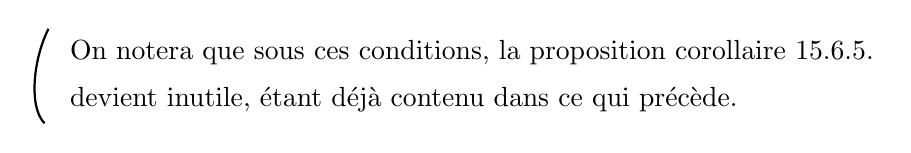
\begin{tikzpicture}[x=1cm,y=1cm]
\node[anchor=west] at (0,0) {On notera que sous ces conditions, la \deleted{proposition} corollaire 15.6.5.};
\node[anchor=west] at (0,-.6) {devient inutile, étant déjà contenu dans ce qui précède.};
\draw[line width=.8pt] (-.15,.3) .. controls (-.35,-.1) and (-.4,-.7) .. (-.2,-.9);
\end{tikzpicture}}

IV 15.6.7. p.241, l. 2, après ``noethérien'' ajouter ``ou si la condition
\figure{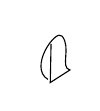
\begin{tikzpicture}[x=1cm,y=1cm]\draw (0,0) .. controls (-.25,.15) and (.1,.65) .. (.18,.55) .. controls (.3,.4) and (.15,.15) .. (.28,.12)--(.03,-.04)--(.04,.45);\end{tikzpicture}}
de 15.6.6. est vérifiée''.

Il convient également d'ajouter quelques points d'\uline{autocritique} (peut-être bloqués ensemble, en C) après les ``modifications de textes), savoir les points suivants:

1º) Suivant une idée de Raynaud, il apparait maintenant qu'on peut traiter de façon nettement plus satisfaisante le contenu des par.14 et 15 en utilisant l'outil de la hensélisation développé au par.18 . De cette façon, on arrive à des formulations et des démonstrations plus simples, tous les résultats principaux étant de plus indépendants de tou-te hypothèse noethérienne. De plus, on arrive à établir aussi par cette voie que la notion de morphisme universellement ouvert \deleted{\unsure{se compor}} de présentation finie se comporte bien par limites projectives de schémas, suivant le point de vue du par.8 . Nous espérons présenter une version entièrement refondue de ces résultats dans la réédition, où \deleted{\unsure{ils apparaîtr}} la substance des actuels par.14 et 15 se trouvera rejetée après le par. 18 (ce qui ne présente aucun inconvénient, les par. 16 et suivants étant visiblement indépendants des actuels par.14 et 15).

2º) Nous nous répentons sincèrement de l'usage immodéré fait du terme ``non \uline{ramifié'' au lieu de ``net''}. Nous pourrions ajouter quelques

\mspage{41}
